\documentclass{report}
\usepackage{titlesec}
\usepackage{titling}
\usepackage{graphicx}
\usepackage{tikz}
\usepackage{pgfplots}
\usepackage{caption}
\usepackage{multirow}


\title{\textbf{UBL201-L Introductory Biology III - Immunology}}
\author{Rahul Chavan - 22086}
\date{12th September 2023}


\usepackage[left=1in, right=1in, top=0.5in, bottom=0.5in]{geometry}
\renewcommand{\maketitle}{
 \begin{center}
    \includegraphics[width=2cm]{IISc_Master_Seal_Black.jpg}
    \vspace{0.5cm}

    \Large
    \textbf{\thetitle}
    
    \vspace{0.5cm}
    
    \Large
    \theauthor
    
    \vspace{0.2cm}
    
    \large
    \thedate

    \vspace{0.5cm}

    \hrule  
    
  \end{center}
}

\pgfplotsset{compat=1.18}
\begin{document}
\maketitle
\begin{center}
    \large
    \textbf{Quantitation of nitric oxide (NO) production by macrophages
in response to different doses of lipopolysaccharide (LPS)}
\end{center} 

%Lab report: 

%•      Title of the experiment 

%•      Principle 

%•      Results and discussion 

%•      Interpretation 

%•      Precautions 

\section*{Principle:} 
Nitric oxide (NO) is a free radical that is produced by the enzymatic conversion of L-arginine to L-citrulline by nitric oxide synthase (NOS).
NO is produced by a variety of cells, including macrophages, in response to inflammatory stimuli such as lipopolysaccharide (LPS).
NO is a potent vasodilator and has been shown to be involved in the pathogenesis of septic shock. Inflammatory stimuli can enhance NO
release via the up-regulation of the inducible form of NOS (iNOS or NOS2) Within inflammatory macrophages.
NO is converted into highly Reactive Nitrogen Species (RNS) such as $NO_{3}^{-}$ and $NO_{2}^{-}$ within infected macrophages
to drive bacterial death. NO is also involved in the regulation of apoptosis and the immune response.


NO production can be measured by the Griess reaction, which is based on the ability of NO to react with sulfanilamide 
and N-(1-naphthyl)ethylenediamine. Sulfanilamide is converted to a diazonium salt by reaction with nitrite( $NO_{2}^{-}$) in acid solution. The diazonium salt 
is then coupled to N-(1-napthyl) ethylenediamine leading to the formation of an azo dye (Pink colour), a chromophore 
that can be measured spectrophotometrically at 540 nm.
The amount of NO produced by macrophages in response to LPS can be quantitated by comparing the absorbance of the sample to a standard curve generated using a known concentration of sodium nitrite.
Using a standard curve, the concentration of NO produced by the macrophages can be determined from the absorbance of an 
unknown sample.
Therefore, using Griess's reagent we can indirectly estimate levels of NO by quantification of nitrite in the biological samples.
 \begin{figure}[htbp]  
   \centering 
   \includegraphics[width=0.7\textwidth]{nitriterxn.jpg} 
   \caption{Reaction of nitrite with Griess reagent}
   \label{fig: Reaction } 
 \end{figure}


\vspace{1cm}

\section*{Results and discussion:}   

\subsubsection*{Absorbance values of serial dilutions of NO2 at 550 nm:}
   \begin{table}[ht]
    \centering
    \caption{Absorbance values of serial dilutions of NO2 at 550 nm}
    \vspace{0.5cm}
    \label{tab:table1}

    \begin{tabular}{|c|c|c|c|c|c|c|c|c|}
      \hline
      \textbf{Concentration of NO2 (µM)} & 208.3 & 104.15 & 52.075 & 26.0375 & 13.01875 & 6.5009 & 3.2505 & \textbf{unknown} \\
      \hline
      \textbf{Absorbance Values for Trial 1} & 2.7295 & 1.4981 & 0.811 & 0.407 & 0.2853 & 0.1093 & 0.0914 & 0.3657  \\
      \hline
      \textbf{Absorbance values for Trial 2} & 3.8812 & 0.4592  & 0.4985 & 0.2243 & 0.2316 & 0.115 & 0.0864 & 0.3733 \\
      \hline
      \textbf{Absorbance values for Trial 3} & 3.8595 & 0.7958 & 0.2099 & 0.1189 & 0.0979 & 0.0957 & 0.0713 & 0.3616 \\
      \hline
    \end{tabular}
  
   \end{table}
\subsubsection*{Absorbance values of the blank at 550 nm:}    
   \begin{table}[ht]
     \centering
      \caption{Absorbance values of the blank at 550 nm}
      \vspace{0.5cm}
      \label{tab:table2}
      
      \begin{tabular}{|c|c|}
        \hline
        \textbf{Concentration of NO2 (µM)} & \textbf{Blank} \\
        \hline
        \textbf{Absorbance Values for Trial 1} & 0.0449  \\
        \hline
        \textbf{Absorbance values for Trial 2} & 0.0451  \\
        \hline
        \textbf{Absorbance values for Trial 3} & 0.00455 \\
        \hline
      \end{tabular}
    \end{table}

In our case the absorbance values for Trials 2 and 3 would give us a parabolic curve and not a 
straight line. In order to infer for the concentrations, we chose the absorbance values of Trial 
1 only, to account for the concentration of the unknown sample.

 \vspace{1cm}

\subsubsection*{Concentration vs Absorbance Table:}
    \begin{table}[h]
      \centering
        \caption{Concentration vs Absorbance Table}
        \vspace{0.5cm}
        \label{tab:table3}
        
        \begin{tabular}{|c|c|}
          \hline
          \textbf{Concentration of NO2 (µM)} & \textbf{Absorbance} \\
          \hline
          208.3 &  2.6846 \\
          \hline
          104.15 & 1.4532  \\
          \hline
          52.075 & 0.7611 \\
          \hline
          26.0375 & 0.3621  \\
          \hline
          13.01875 & 0.2404  \\
          \hline
          6.5009 & 0.0644 \\
          \hline
          3.2505 & 0.0465 \\
          \hline
        \end{tabular}
      \end{table}
Here, the new absorbance values are obtained by subtracting the absorbance value of the 
blank from the original values (values are from Trial 1 only).

\subsubsection*{Concentration vs Absorbance Graph:}
\begin{center}


   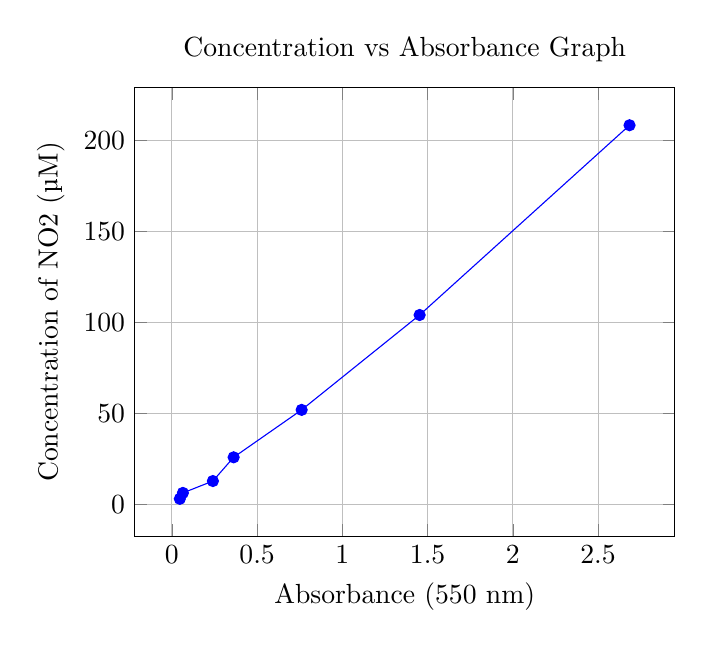
\begin{tikzpicture}
      \begin{axis}[
      xlabel={Absorbance (550 nm)},
      ylabel={Concentration of NO2 (µM)},
      title={Concentration vs Absorbance Graph},
      grid=major,
     ]
      \addplot[color=blue,mark=*] coordinates {
      (2.6846,208.3)
      (1.4532,104.15)
      (0.7611,52.075)
      (0.3621,26.0375)
      (0.2404,13.01875)
      (0.0644,6.5009)
      (0.0465,3.2505)

     };
      \end{axis}
  \end{tikzpicture}

\end{center}

 \vspace{1cm}

\subsubsection*{Linear fitting of the plot:}
\begin{figure}[htbp] 
  \centering 
  \includegraphics[width=0.7\textwidth]{no2.jpg} 
  \caption{Linear fitting of the plot}
  \label{fig: Linear fitting} 
\end{figure}



Using the plot, we can determine the concentration of the unknown sample:

As we know : y = mx + b

where, y = concentration of NO2 (µM)

x = absorbance (550 nm)

m = slope of the line

b = y-intercept

For the unknown, 
x = 0.3208 

from the plot we get, m = 77.2 and b = -2.92

therefore, y = 21.84576 

Hence, the nitric oxide concentration of the unknown sample using Griess reagent assay is 21.84576 µM.

 \vspace{2cm}




\section*{Interpretation:}
From the plot we can see that there exists a linear realtionship between the concentration of NO2 and the absorbance values.
As we know that more is the LPS dosage to the cells, more is nitrite production, we can also establish that more LPS dosage samples will give higher absorbance values.
The blank as expected gave negligible absorbance values as it does not contain any nitrite.
However, due to pippeting errors, the difference in the absorbance values of duplicates and triplicates is significantly high. Hence, we 
cannot rely on the values of the duplicates and triplicates. We can only rely on the values of the first trial.

Using the data we can conclude that nitric oxide concentration of the unknown sample using Griess reagent assay is 21.84576 µM
i.e., it lies between the $4^{th}$ and $5^{th}$ diluted concentrations which are 26.0375 µM and 13.01875 µM respectively, 
implying the source cells were subjected to a lower concentartion of LPS dosage or the cells were not able to produce enough nitric oxide due 
to lower activation.


\section*{Precautions:}

\begin{itemize}
  \item Wear appropriate personal protective equipments, including lab coats, gloves, and safety goggles,
         to protect against chemical exposure.
  \item Use sterile techniques and clean glassware to prevent contamination of samples and reagents.
  \item Calibrate and standardize the spectrophotometer using appropriate standards and 
         controls to ensure accurate measurements.
  \item Avoid pippeting errors and ensure that the pippetes are calibrated.
  \item Avoid exposure to light, as Griess reagent is light-sensitive.
  \item Perform duplicates and triplicates to reduce the error and enhance reproducibility of results.
  \item Careful disposal of bioharzardous waste.
\end{itemize}



\end{document}